\documentclass{article}
\usepackage[utf8]{inputenc}

\title{Software Design 2014 Final Report - Get A Room}
\author{Dimitar Dimitrov and Kyle Flores}
\date{May 2014}

\usepackage{graphicx}
\usepackage{placeins}

\begin{document}
\maketitle

\section*{Final Design}
\subsection*{Flow and Method}
\FloatBarrier
\begin{figure}[h!]
    \centering
    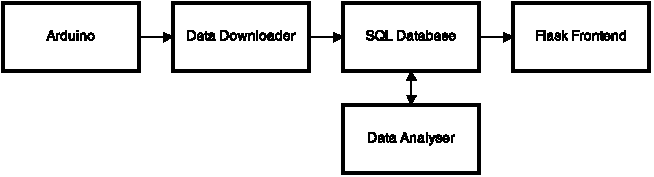
\includegraphics[scale=0.75]{flowpicture.pdf}
    \caption{Flow diagram}
\end{figure}
\FloatBarrier
\par The general flow of information through the system has remained consistent throughout the project, while the method around it has changed. Each sensor hosts a webpage where it reports all relevant data. A python script connects to all known sensor webpages and downloads the data they host, then organizes it into a SQLite database. A Flask web app reads the database directly for real time data, and another script reads the database to analyze historical data, which is also hosted on the web app.

\subsection*{Data Structures}
\par This product uses a mix of Python data structures to move data internally. For example, the Arduino hosted webpages format sensor values in a string that looks like a dictionary so that it can be parsed easily by the built-in module, ast.  The key to this dictionary is the sensor's name, and the value is the sensor value. This is convenient because fields are named after the sensor, and it is easy to match datatable fields with dictionary keys.
\par Information about each sensor node and sensor values at a certain time are encapsulated in "Node" or "data" classes.  Abstracting the sensors and data values as objects is convenient because it allows data to be easily linked to the sensor it came from. It also allows us to store important information about the sensors, such as their physical location or ip address, as class attributes. Finally, SQLAlchemy writes rows to tables by assigning objects, so using an object oriented approach allows simple integration.
\par All historical data is stored to a SQLite database because SQL provides a much cleaner and robust way of accessing large amounts of data than simply writing a csv file.  While a csv, numpy dtype, or pickle would have likely worked for the current scope of the project, using SQLite was determined to be the best approach in the interest of Flask integration and general scalability.

\subsection*{UML Diagram}
\FloatBarrier
\begin{figure}[h!]
    \centering
    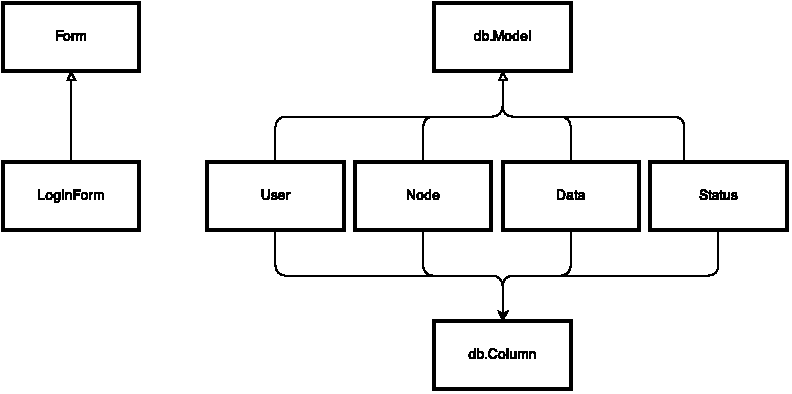
\includegraphics[scale=0.75]{UML.pdf}
    \caption{UML diagram}
\end{figure}
\FloatBarrier

\section*{Results}
\par The product we presented during the class demo-day was something we were proud to put our names on. Because we reached our minimum deliverable relatively early in the project, our product incorporated some of the features we scoped out intially as extensions, and shows some refinement towards our design criteria
\begin{itemize}
 \item Detects when the door in a room is opened.
 \item Reports light and temperature values.
 \item Sensor kit servers secure a static IP address on the network.
 \item Data is stored to a SQLite database which is more certainly more robush than a csv.
 \item Flask integrates with SQLite and hosts a webapp on LAN that lets users view historical and current data
 \item Databases can be updated to accomodate new sensor nodes and sensor types without needing to reset the original databse.
 \item All configuration changes can be made without modifying source: Adding new sensor nodes requires modifying a "config.txt file" and migrating databases involves running a couple of python scripts.
\end{itemize}
Although in a software project, it is also possible to add more features, improve source maintainability, or beautify UI elements, we were satisfied with what we accomplished in the time alotted, considering also that we had a hardware component to work with, and learned to work with SQL and Flask independently.

\section*{Division of Labor}
\par The first step of our project, networking hardware, was difficult to work on in parallel because all downstream elements depended on it. Until we had the Arduino sensor kits installed and network enabled, we could not write data acquisition scripts and it was difficult to determine how to create reasonable databases. We were able to write different aspects of the data acquistion routine in parallel however. The downloading from a webpage, webpage parsing, and data storage could be written independently provieded the input and output formats were known, which we did a decent job of documenting and keeping consistent. We later moved on to writing SQL models and the Flask app in parallel until the two were mature enough to be integrated. While this project was relatively large in scope for two people, our small team size ended up being appropriate.

\section*{Bugs and Troubleshooting}
\par The worst kind of bugs are hardware bugs. We spent an absurd amount of time trying to figure out why our Arduino and ethernet controller would lose network connection at random times. After testing for Arduino C bugs, hardware connection issues, and ethernet port issues, we eventually discovered that the ENC28J60 breakout we were using was known to overheat on occasion due to poor board design. The problem was solved by taping a penny to the chip to help dissipate heat. 

\par Because neither of us had any experience with SQL prior to this project, SQLalchemy was at first unintuitive and tutorials were difficult to follow. Code we wrote to implement SQLite for our purposes was of course, difficult to debug too. Solutions were eventually found to most of the problems by iterative testing.

%\par Dimitar, you probably want to say something about Flask or web hosting here.
\section*{Design Reflection and Future Extensions}
\par In retrospect, several aspects of the design were not optimal, and should be reconsidered if the project were to be extended.  Additionally, certain features we wish were present didn't quite make it, or weren't mature: they are listed here as well.
\begin{itemize}
    \item Sensor webservers should have two way communication with the main server that runs the web app and database. If sensors could send information to the server rather than the server requesting it, sensor IP addresses could be populated autonomously, and the sensors would not require modification of Arduino source code. Additionally, if the main server could send information to the sensors, it could report its own configuration as well.
    \item The analysis routine, or at least a placeholder for the analysis routine, should have been developed earlier in the development cycle. It was impossible to deliver a mature analysis of whether the room was occupied or not before all sensors were accounted for, and a reasonable amount of data was collected. This is more of a planning and foresight mistake than a design mistake.
    \item To make this system even more general and extend its possible applications, the software should have been designed to automatically SQL tables and columns based on the data it pulls up from sensors.  Right now, "temperature","light","door", etc values are all written directly into the source and cannot be modified.
%    \item Dimitar add anything else you think is relevant.
\end{itemize}

\section*{Closing Remarks and Acknowledgements}
We would like to thank the Software Design 2014 course assistants, especially Joshua Langowitz and Amun Kapur for their guidance.  We hope that Aman enjoys a large ASCII picture of him in /app/models.py. We would of course like to thank Professor Paul Ruvolo as well for his guidance and for a positive learning experience in this class.
\end{document}
